% interacttfqsample.tex
% v1.05 - August 2017

\documentclass{interact}
\usepackage[caption=false]{subfig}
%\usepackage[nolists,tablesfirst]{endfloat}% To `separate' figures and tables from text if required
%\usepackage[doublespacing]{setspace}% To produce a `double spaced' document if required
\usepackage{graphicx}
\usepackage{amsmath}
\usepackage{url}
\usepackage{tikz}
\usetikzlibrary{shapes.callouts, positioning, arrows.meta, calc, decorations.pathreplacing}
\usepackage[breakable]{tcolorbox}

\usepackage[numbers,sort&compress]{natbib}
\bibpunct[, ]{[}{]}{,}{n}{,}{,}
\renewcommand\bibfont{\fontsize{10}{12}\selectfont}
\setcounter{secnumdepth}{2}
\theoremstyle{plain}
\newtheorem{theorem}{Theorem}[section]
\newtheorem{lemma}[theorem]{Lemma}
\newtheorem{corollary}[theorem]{Corollary}
\newtheorem{proposition}[theorem]{Proposition}
\theoremstyle{definition}
\newtheorem{definition}[theorem]{Definition}
\newtheorem{example}[theorem]{Example}
\theoremstyle{remark}
\newtheorem{remark}{Remark}
\newtheorem{notation}{Notation}
\newcommand{\model}[1]{\texttt{#1}}
\usepackage{xspace}
\newcommand{\Threshold}{\textbf{\texttt{Threshold}}\xspace}
\newcommand{\Surplus}{\textbf{\texttt{Surplus}}\xspace}
\definecolor{figblue}{HTML}{3B82F6}
\definecolor{figred}{HTML}{EF4444}

\begin{document}

\articletype{Research Article}% Specify the article type or omit as appropriate

\title{Quality over Closure in Agentic Supply Chains: BATNA-Aware Reward Design for LLM Buyer--Supplier Negotiation}


\author{
\name{Dhruv Bansal \textsuperscript{a}, Rui Yin \textsuperscript{b}, and Yalin Wang \textsuperscript{a}}
\affil{\textsuperscript{a} School of Computing and Augmented Intelligence, \\Arizona State University, Tempe, AZ, USA \\
\textsuperscript{b} NASPRO Department of Supply Chain Management, \\ Arizona State University, Tempe, AZ, USA
}
}

\maketitle

\begin{abstract}
Negotiation is a core procurement mechanism for determining prices, allocations, and contract terms when private information is present. As artificial intelligence moves from decision support to autonomous agency, buyer--supplier bargaining can increasingly be delegated to software that converses, reasons over constraints, and commits to offers at scale. This shift creates a governance problem: an agent optimized merely to close deals may accept contracts a manager would reject relative to the firm's Best Alternative to a Negotiated Agreement (BATNA). We address this problem by designing BATNA-aware rewards for large language model negotiation agents. The reward introduces a tunable utility floor that represents a package-level resistance point, penalizes agreements below that floor, and is applied selectively to multi-item negotiations where no natural structural floor exists, while surplus rewards are retained for price bargaining. We train a single unified agent across four price and multi-item benchmarks and evaluate it against both its frozen training opponent and stronger frontier models, including transfer to a held-out hybrid task. The proposed reward achieves the highest average bargained ratio, reduces deal-closing bias, and offers an interpretable control for agentic procurement systems.
\end{abstract}

\begin{keywords}
Procurement negotiation; supply chain management; agentic supply chain; autonomous negotiation agents; large language models; Best Alternative to a Negotiated Agreement; reward design; reinforcement learning
\end{keywords}


\section{Introduction}\label{sec:intro}

Procurement negotiation is not simply a search for agreement. In managerial practice, a buyer prepares for a supplier negotiation by clarifying its interests, translating multi-issue preferences into a comparable scoring system, identifying its Best Alternative to a Negotiated Agreement (BATNA), setting a resistance point below which agreement is worse than no agreement, and diagnosing whether the encounter is primarily distributive or integrative \cite{fisher1981gettingtoyes,raiffa1982art,hames2012negotiation,lewicki2010negotiation}. These acceptance rules also vary by sourcing context: Kraljic's purchasing portfolio distinguishes leverage, strategic, bottleneck, and noncritical categories, implying that a buyer's walk-away posture should reflect both value potential and supply risk \cite{kraljic1983purchasing}. These concepts are basic because they determine delegation authority: a procurement manager can authorize a negotiator to pursue a contract only after specifying what counts as an acceptable package of terms and when the negotiator should walk away. Deal closure, by itself, is therefore not a success metric. A contract that falls below the buyer's outside option destroys value even if it is mutually signed.

\begin{figure}[!tbp]
\centering
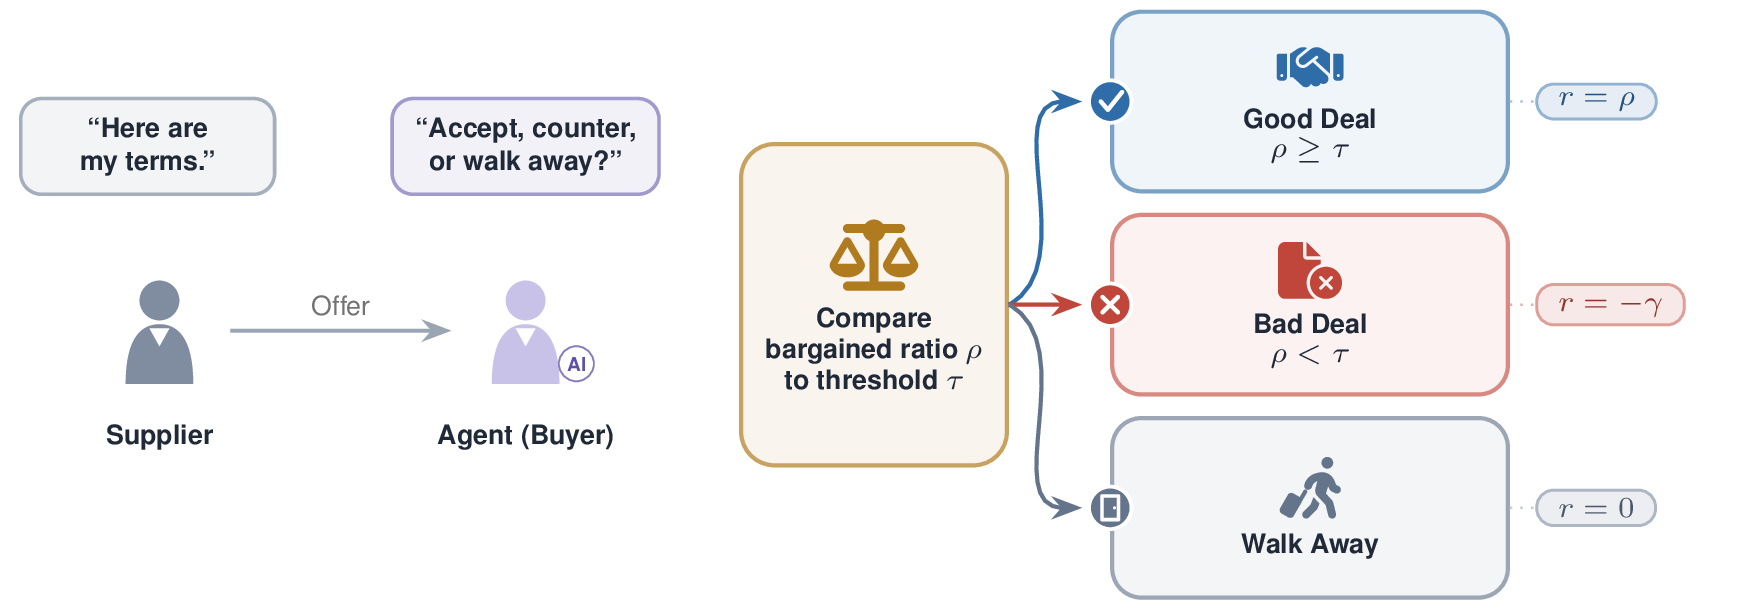
\includegraphics[width=1\columnwidth]{figures/fig1_hero.png}
\caption{BATNA-aware reward design for autonomous negotiation agents.
The agent evaluates each proposed agreement against a quality threshold
$\tau$ that represents the buyer's package-level resistance point. Deals
at or above the threshold are rewarded by their bargained value, deals
below the threshold are penalized, and walking away remains preferable
to accepting an agreement worse than the outside option.}
\label{fig:hero}
\end{figure}

Supply chains are entering an agentic era in which autonomous software agents, rather than human staff, increasingly execute the operational decisions that move goods and money between firms \cite{revilla2023ai,menache2025generative}. The question of whether software agents could automate inter-firm coordination predates the current generation of models \cite{xu2021bots}, but large language models (LLMs) with broad reasoning and language competence \cite{bubeck2023sparks} have sharply expanded what such agents can do, and recent work has begun to deploy them for autonomous, multi-agent coordination across supply chain functions \cite{jannelli2024agentic,li2025chatsync}. Procurement is among the first functions to feel this shift: routine purchasing, supplier selection, and contract bargaining can now be delegated to LLM agents that read a request for quotation, reason about terms, and negotiate with suppliers in natural language. The promise is substantial. A single agent can run thousands of parallel negotiations across a long-tail supplier base that no human team could service, applying a consistent strategy at a marginal cost approaching zero. Yet the same autonomy makes failures consequential and silent. An agent that systematically concedes too much, or closes contracts it should have declined, can erode procurement margins across an entire category before any human reviewer notices.

This makes reward design a managerial governance problem, not only a machine learning problem. A human buyer enters the negotiation with a reservation price, a package-level resistance point, and an understanding of the organization's alternatives. An autonomous buyer must carry the same discipline in the objective used to train it. If its reward treats every signed contract as better than no deal, the agent is being trained to value closure even when a procurement manager would reject the offer. The central question for agentic procurement is therefore not whether an LLM can negotiate, but whether its learned strategy respects the same BATNA-aware acceptance rule that governs sound buyer--supplier bargaining.

This managerial concern is visible in recent negotiation-agent research. Benchmarks for LLM negotiators across price bargaining and multi-item allocation show that even frontier models routinely accept negative-utility deals \cite{xia2024measuring, kwon2024llmseffectivenegotiators, bianchi2024negotiationarena, noh2024personalities, chatterjee2024agreemate, hua2024gametheoretic}. Reinforcement learning has been used to improve strategic behavior \cite{liu2026instructing, bergemann2026bilateral, vendrell2026gametalk, zeng2025repo, long2025evoemo, oh2026merit}, but existing methods typically train on a single task type and rely on surplus rewards that treat any closed deal as positive. The missing managerial principle is the BATNA-based walk-away rule: rational negotiators should prefer no agreement to any agreement worse than their outside option. In supply chain terms, an agent without such a rule is a buyer without a credible reservation point, and a buyer who will accept any contract is a buyer that suppliers can exploit.

% \begin{figure}[!tbp]
% \centering
% \begin{tikzpicture}[
%   scale=0.85, every node/.style={scale=0.85},
%   >=Stealth,
%   agent/.style={
%     rectangle, rounded corners=6pt, draw=black, fill=white,
%     minimum width=2.2cm, minimum height=1.4cm, align=center,
%     font=\small\bfseries
%   },
%   thought/.style={
%     ellipse callout, draw=orange!50, fill=orange!8,
%     callout relative pointer={(#1)},
%     font=\scriptsize, align=center, inner sep=4pt
%   },
%   deal/.style={
%     rectangle, rounded corners=4pt, draw=figblue!60, fill=figblue!8,
%     minimum width=1.6cm, minimum height=0.9cm, align=center,
%     font=\scriptsize
%   },
%   bad/.style={
%     rectangle, rounded corners=4pt, draw=figred!60, fill=figred!8,
%     minimum width=1.6cm, minimum height=0.9cm, align=center,
%     font=\scriptsize
%   },
%   walk/.style={
%     rectangle, rounded corners=4pt, draw=black!40, fill=gray!10,
%     minimum width=1.6cm, minimum height=0.9cm, align=center,
%     font=\scriptsize
%   },
%   reward/.style={font=\scriptsize\bfseries},
% ]

% \node[agent] (agent) {Negotiation\\Agent};

% \node[thought={(-1.2cm, -0.8cm)}, above right=1.0cm and 0.4cm of agent]
%   (bubble) {Which is better?};

% \node[deal, above right=0.2cm and 2.8cm of agent] (good)
%   {Good Deal\\$\rho \geq \tau$};
% \node[reward, right=0.3cm of good, figblue!80!black] {$r = \rho$};

% \node[bad, right=2.8cm of agent] (bad)
%   {Bad Deal\\$\rho < \tau$};
% \node[reward, right=0.3cm of bad, figred!80!black] {$r = -\gamma$};

% \node[walk, below right=0.2cm and 2.8cm of agent] (walk)
%   {Walk Away};
% \node[reward, right=0.3cm of walk, black!50] {$r = 0$};

% \draw[->, thick, figblue!80!black]
%   (agent.east) ++(0.15,0.3) -- (good.west);
% \draw[->, thick, figred!60, dashed]
%   (agent.east) ++(0.15,0) -- (bad.west);
% \draw[->, thick, black!40]
%   (agent.east) ++(0.15,-0.3) -- (walk.west);

% \end{tikzpicture}
% \caption{Training the agent to incorporate the best-alternative
% principle by enforcing an abstract quality threshold $\tau$
% rather than accepting sub-optimal deals.}
% \label{fig:batna_hero}
% \end{figure}



The correct reward, however, depends on the structure of the negotiation. Price bargaining is primarily distributive: the buyer and supplier divide a fixed monetary surplus, and the supplier's reservation price creates a natural floor on deal quality. Multi-item and multi-attribute contracting is closer to an integrative package negotiation: the parties trade across issues with different private priorities, and the relevant acceptance rule applies to the package as a whole rather than to any single issue. In these settings, a counterpart can steer the agreement toward a jointly feasible but badly lopsided package, and surplus-only rewards create a deal-closing bias in which agents optimize for agreement rather than agreement quality \cite{bergemann2026bilateral}. The managerial implication is selective rather than universal: a BATNA-aware penalty is most needed where the task lacks a structural quality floor, while applying the same penalty to every thin-margin price deal would overdiscipline legitimate agreements.

We operationalize this idea as a threshold reward for LLM negotiation agents. Figure~\ref{fig:hero} summarizes the decision logic: the agent is not rewarded for closure alone, but compares the agreement's bargained ratio with a managerial quality threshold before accepting. The threshold is a tunable quality floor that represents the buyer's package-level resistance point: closed deals above the floor are rewarded by their bargained value, closed deals below it are penalized, and walking away remains preferable to accepting a poor agreement. We apply this signal selectively to multi-item settings while retaining surplus rewards for price bargaining, then train a single agent across four benchmarks spanning both task types and evaluate it on a held-out fifth dataset. Our contributions are threefold: (1) we provide a practical reinforcement-learning framework for developing customized LLM negotiation engines, in which an organization's bargaining policy can be encoded as verifiable rewards and local guardrails; within this framework, we translate the BATNA/resistance-point logic of negotiation management into one concrete reward design for autonomous buyer agents; (2) we show that reward design should be matched to negotiation structure, distinguishing single-issue price bargaining from multi-issue package negotiation; and (3) we validate the system across five distinct benchmark datasets, demonstrating improved deal quality, reduced deal-closing bias, and transfer to an unseen negotiation structure compared with both surplus-based training and frontier LLM baselines. Together, these contributions position quality-over-closure not as the only possible objective, but as an example of how business negotiation principles can be turned into trainable controls for future customized and private negotiation agents.

The paper, therefore, speaks to both reinforcement learning and supply chain management. For RL, it shows that the strategic behavior of negotiation agents depends critically on the economic meaning encoded in the terminal reward, not merely on the choice of training algorithm. For procurement, it offers a governance mechanism: managers can express how aggressively an autonomous buyer should hold out for better terms through a single interpretable quality threshold, rather than delegating bargaining authority to a black-box agent optimized for closure. The remainder of the paper reviews the relevant literatures (Section~\ref{sec:related}), formalizes the negotiation setting, benchmarks, MDP formulation, and selective reward design (Section~\ref{sec:method}), reports experiments against both a fixed and a stronger frontier opponent (Section~\ref{sec:results}), and develops the managerial implications for supply chain procurement (Sections~\ref{sec:discussion}--\ref{sec:conclusion}).


\section{Related Work}\label{sec:related}

Negotiation research has long treated bargaining as a managerial process of preparation, structural diagnosis, and disciplined agreement selection. Classical accounts combine formal bargaining theory with the practical logic of principled negotiation: negotiators prepare by clarifying interests, diagnosing whether the setting is distributive, integrative, or mixed, identifying their BATNA, and remaining willing to walk away when the proposed agreement fails to beat that alternative~\cite{nash1950bargaining,fisher1981gettingtoyes,raiffa1982art,lewicki2010negotiation}. In supply chains, these principles become operational because buyer--supplier negotiations shape contract terms, relationship quality, and performance~\cite{hames2012negotiation}. Single-issue price bargaining is primarily distributive, while multi-issue contracts can create value through trade-offs across privately weighted terms~\cite{davis2019multidimensional,haruvy2020bargaining}. At the sourcing-portfolio level, Kraljic's matrix classifies purchases by profit impact and supply risk into leverage, strategic, bottleneck, and noncritical categories, making negotiation posture a function of category context rather than a universal rule~\cite{kraljic1983purchasing}. Leverage categories, where buyer alternatives are stronger, can support more assertive value-capture thresholds; bottleneck categories call for continuity-preserving thresholds; and strategic categories require balancing value capture against relationship preservation and supply assurance. Power asymmetry and supply-market concentration further determine how aggressively buyers can hold to their walk-away thresholds~\cite{kaufmann2004mode,nyaga2013power}. This literature establishes the management baseline for our work: a negotiated agreement is valuable only when it is better than the buyer's outside option, and the correct strategy depends on the negotiation's structure and sourcing context.

Recent advances in AI move this negotiation logic into a new operational setting. The agentic-supply-chain vision imagines autonomous systems that perceive, reason, use tools, coordinate with other agents, and act across procurement, planning, logistics, and fulfillment. This vision builds on older agent-based supply chain automation~\cite{xu2021bots}, but LLMs have renewed the agenda by making language-based reasoning and planning broadly accessible~\cite{bubeck2023sparks}. Current work highlights opportunities in supply chain planning and decision support~\cite{menache2025generative}, multi-agent consensus seeking~\cite{jannelli2024agentic}, and production logistics synchronization~\cite{li2025chatsync}, while also warning that LLMs can reproduce managerial biases rather than eliminate them~\cite{chen2025manager}. The implication for supply chain management is that agentic AI is not merely another optimization tool; it is a delegation technology whose behavior must be aligned with managerial intent.

Negotiation is a particularly demanding form of such delegation because it is sequential, adversarial, and conducted under private information. Commercial systems already automate standardized supplier negotiation~\cite{revilla2023ai}, and LLM agents have been proposed both as operational negotiators and as behavioral surrogates for human bargainers~\cite{kirshner2024artificial,bianchi2024negotiationarena,yin2026negotiation}. Early neural negotiation models studied multi-item allocation and price bargaining~\cite{lewis2017deal,he2018decoupling}, and recent LLM benchmarks broaden the setting to price, personality, game-theoretic, and multi-agent negotiation tasks~\cite{xia2024measuring,kwon2024llmseffectivenegotiators,noh2024personalities,chatterjee2024agreemate,hua2024gametheoretic}. These studies show that LLMs can conduct fluent negotiation, but fluency is not the same as competence: models may accept negative-utility deals, open too close to their reservation point, or lose to simple predefined tactics. The managerial problem is therefore not whether an agent can produce plausible bargaining dialogue, but whether it can be trained to make economically disciplined accept, reject, and walk-away decisions.

Reinforcement learning is a natural approach for this problem because negotiation quality is realized through multi-turn interaction rather than one-shot prediction. Recent work shows that RL and related feedback methods can elicit richer bargaining behavior, including anchoring, persuasion, and strategic adaptation~\cite{liu2026instructing,vendrell2026gametalk,zeng2025repo,long2025evoemo,oh2026merit}. Reinforcement learning from verifiable rewards is especially attractive because final contracts can often be scored from structured deal terms without human preference annotation~\cite{liu2026instructing,shao2024deepseekmath}. Yet the reward itself remains underdeveloped. Existing studies often train on a single task family and reward any positive closed deal, which can create a deal-closing bias in which agents optimize for agreement rather than agreement quality~\cite{bergemann2026bilateral}. This gap motivates the present work. We design a BATNA-aware reward that teaches agents to prefer walking away to accepting low-quality agreements, and we apply it selectively across heterogeneous price and multi-item benchmarks so that the reward design reflects the negotiation's structure rather than imposing a universal closure objective.

\section{Methodology}\label{sec:method}

We introduce our methodology in four steps. First, we map five dialogue benchmark datasets into two procurement-relevant negotiation families: single-issue price bargaining and multi-item or multi-attribute package negotiation. Second, we cast every benchmark as the same finite-horizon interaction problem, with a learner that observes its own private constraints, exchanges offers with a frozen opponent, and chooses among structured bargaining actions. Third, we score each terminal contract using a normalized bargained ratio, so that monetary prices, item allocations, and held-out job-offer attributes can be compared on a common scale. Fourth, we compare two terminal reward designs: a surplus reward that values any closed agreement and a BATNA-aware threshold reward that penalizes low-quality multi-item agreements while leaving price bargaining on its natural surplus scale. The experimental section (Section~\ref{sec:results}) then uses this common interface to train and evaluate a single policy across heterogeneous negotiation structures.

\subsection{Negotiation Setting and Benchmarks}\label{sec:benchmarks}

A bilateral negotiation is the atomic transaction of a supply chain: two self-interested parties, such as a buyer and a supplier, must agree on the terms of an exchange before any goods or commitments change hands. Each party holds private information, a reservation value below which the exchange is not worth making, and neither can see the other's. They proceed in rounds, alternating offers and counteroffers, and at each turn a party may concede, hold firm, accept the standing offer, or walk away to its \emph{outside option}, the best alternative available if no agreement is reached. Negotiation is therefore not a one-shot optimization but a sequential, information-asymmetric process under a deadline, and a competent agent must trade off the risk of impasse against the cost of conceding. The quality of an agreement is how much of the available surplus a party secures relative to its outside option, so accepting a deal worse than walking away is a strictly losing move, the failure our reward design targets.

What is being negotiated separates our benchmarks into two families with a structurally decisive difference: whether the agreement space has a natural quality floor. In \emph{price bargaining}, the parties settle a single scalar price, the unit price a buyer pays a supplier. Because no rational supplier sells below its cost, the price is bounded from below and the buyer's worst closed deal is still floored by that reservation. In \emph{multi-item allocation} the parties divide a fixed bundle of goods, the composition of an order or the split of constrained shared resources, over which each side holds private valuations. Here, a cooperative counterpart can accept a split that leaves the learner almost nothing, and no reservation price rules out an agreement worse than the outside option. This asymmetry is the empirical motivation for the selective reward design of Section~\ref{sec:reward}. We train on four datasets spanning both families and reserve a fifth dataset for transfer testing.

\paragraph{Price bargaining}
These datasets cast the learner as a buyer haggling over a unit price, the canonical procurement interaction. \textbf{AmazonHistoryPrice} (AHP; \cite{xia2024measuring}) pairs a buyer with a seller over real product listings drawn from Amazon price histories; the buyer holds a private budget (its willingness to pay) and the contract reduces to a single agreed price, mirroring catalog procurement against a fixed supplier quote. \textbf{CraigslistBargains} (CRA; \cite{he2018decoupling}) draws from Craigslist postings spanning housing, electronics, and vehicles, where buyer and seller haggle down from a public list price, as in open-market or spot sourcing, where the supplier advertises an anchor and the buyer must extract concessions. In both, deal quality is the buyer's surplus relative to its budget, and the seller's cost floors how low quality can fall.

\paragraph{Multi-item allocation}
These datasets require the parties to partition a fixed set of heterogeneous items, the supply-chain analog of negotiating the composition of an order or dividing constrained shared capacity among partners. \textbf{CaSiNo} (CA; \cite{chawla2021casino}) casts the two parties as campers dividing a shared pool of food, water, and firewood, each holding a private priority ranking that sets its value for each resource; structurally this is the allocation of scarce common materials between two stakeholders with competing internal priorities. \textbf{Deal or No Deal} (DnD; \cite{lewis2017deal}) presents a set of books, hats, and balls with private per-item point values, and a valid contract must assign every item to one side or the other, much like the line-by-line division of a fixed lot or contract whose components are worth different amounts to each party. Because both parties draw private valuations over the same goods, these tasks are structurally symmetric and admit lopsided agreements that no reservation price excludes.

\paragraph{Held-out evaluation}
\textbf{Job Interview} (JI; \cite{yamaguchi2021dialogue}) is withheld from training and used only for evaluation. An applicant and a recruiter negotiate over five issues that combine a salary-like scalar with categorical attributes such as workplace, role, and days off, each side weighting the issues by a private preference profile. Because it mixes a scalar issue with categorical choices, JI matches neither training family exactly, so we use it to measure whether a policy trained on price and allocation tasks transfers to a structure it never saw.

\subsection{MDP Formulation}

We model each negotiation as a finite-horizon Markov Decision Process (MDP) defined as $(\mathcal{S}, \mathcal{A}, \mathcal{P}, R, T)$, where $\mathcal{S}$ is the set of dialogue states, $\mathcal{A}$ the set of negotiation actions, $\mathcal{P}$ the transition kernel, $R$ a terminal reward, and $T$ the per-agent turn horizon. This formulation gives the heterogeneous benchmarks a common structure while preserving their task-specific contract spaces and private constraints.

The learner's policy $\pi_\theta$ is the only one trained; the opponent is a frozen language model absorbed into $\mathcal{P}$, so from the learner's perspective, the counterpart is part of a stationary environment. Since the reward is realized only at termination, the agent optimizes undiscounted return over the horizon and no discount factor is needed.

The opponent's private information is never observed, so the underlying game is formally partially observable; rather than maintain an explicit belief state, we optimize directly over the learner's observed interaction history, which is a sufficient statistic for its own decisions. The objective is not merely to close a deal but to maximize expected terminal utility, accepting an agreement only when it beats the learner's outside option. This outside-option criterion is what we operationalize through a parameterized quality threshold.

Casting negotiation as an MDP rather than a one-shot decision is essential to the procurement framing. A buyer's bargaining power resides precisely in the sequence of moves available to it, namely the ability to open with an aggressive anchor, to concede gradually while reading the supplier's responses, and to credibly threaten to walk away as the deadline approaches. A model that treats negotiation as a single accept-or-reject classification discards this structure and cannot learn the timing of concessions that distinguishes a skilled buyer from a naive one. The finite horizon $T$ encodes the deadline pressure ubiquitous in real procurement, where both parties face the opportunity cost of a protracted negotiation, and the terminal-only reward reflects the fact that what ultimately matters is the contract signed, not the rhetoric that produced it. Because the opponent is frozen and absorbed into the transition kernel, the learner faces a stationary, if unknown, environment, and the learning problem is well-posed: the policy must discover, through repeated play, which sequences of offers extract the most surplus from a counterpart whose reservation it can only infer.

\paragraph{State space}
A state $s_t \in \mathcal{S}$ collects everything the learner can condition on at turn $t$, written $s_t=(d, c_i, h_t, o_t, \ell_t)$. The task description $d$ fixes the goods at stake and the rules of the encounter. The private constraints $c_i$ encode the learner's economic preferences and are what make two structurally identical dialogues call for different moves. The public history $h_t$ is the running record of utterances and offers that keeps the state Markovian, since it summarizes every payoff-relevant event so far. The standing offer $o_t$ is the single contract currently on the table. The turn budget $\ell_t$ measures remaining bargaining power. 

The private component is task-specific. In price bargaining, it is the buyer's maximum willingness to pay $\mathcal{B}$, while in multi-item allocation, it is a vector of item values or preference weights. The counterpart's constraints, the seller's cost $\mathcal{C}$ or the partner's valuations, are deliberately excluded to reproduce the information asymmetry that defines real negotiation: the learner must infer the opponent's reservation from its behavior.

\paragraph{Action space}
Following He et al.~\cite{he2018decoupling}, each action $a_t \in \mathcal{A}$ has three parts: a private thought that is hidden from the opponent and supports multi-step reasoning, a visible utterance that carries the persuasive content of the move, and a structured formal action that the environment can score. The formal action is one of \textbf{Submit Deal}, \textbf{Accept Deal}, \textbf{Reject Deal}, or \textbf{Walk Away}. 

\textbf{Submit Deal} is a scalar price in AHP and CRA and a complete item or attribute allocation in CA, DnD, and JI; \textbf{Accept Deal} commits to the standing offer $o_t$; \textbf{Reject Deal} declines without ending the encounter; and \textbf{Walk Away} terminates with no agreement, the explicit realization of the outside option. Role assignment follows the structure of each benchmark rather than a single convention. In the price datasets, deal quality is measured from the buyer's surplus and only the buyer holds a budget constraint, so we fix the learner as the buyer to keep the trained skill and the evaluation metric on the same side of the market. CA and DnD are structurally symmetric, with both parties drawing private valuations over the same items, so we assign the learner's role at random. In Job Interview, the applicant carries the five-issue preference profile and is the natural focal negotiator, so the learner always plays the applicant.

Appendix~\ref{app:prompts} reports the role prompts behind this interface. This is important for replication and interpretation because the prompts specify where private budgets, costs, item values, and preference weights enter the agent's context, and because the \texttt{Thought}/\texttt{Talk}/\texttt{Action} format is the mechanism that separates private reasoning from the visible offer that can bind the negotiation.

\paragraph{Transition and environment}
The transition kernel $\mathcal{P}$ couples deterministic bookkeeping with the stochastic reply of the frozen opponent. After the learner acts, the environment validates the structured action, updates $h_t$ and $o_t$, decrements the turn budget, and either reaches a terminal state or queries the opponent, whose reply passes through the same contract validator before $s_{t+1}$ is formed. 

Three design decisions keep these dynamics faithful to negotiation rather than to the simulator's artifacts. \emph{Verifiable action interface}: malformed actions receive a penalty and never become usable contracts, which enforces the structured interface that makes the reward verifiable. \emph{Deal regulation}: a regulation step intercepts opponent moves that would hand the learner a negative-utility deal and converts them into rejections; without it, the learner could farm reward by goading an irrational counterpart into self-defeating concessions, and the policy would learn exploitation rather than bargaining. \emph{Bounded termination}: episodes end on agreement, walk-away, repeated rejection loops, or after $T{=}6$ rounds per agent, so that stalling is bounded and the terminal reward is always well-defined.

\subsection{Reward Design}\label{sec:reward}

The reward depends only on the final contract and the learner's private constraints, so it needs neither a learned reward model nor human annotation. We score a closed deal by its \emph{bargained ratio} $\rho$, the share of available surplus that the learner captures, normalized so that $\rho = 1$ marks the best attainable deal. Let $\mathcal{B}$ denote the buyer's budget, $P$ the agreed price, and $\mathcal{C}$ the seller's cost in price bargaining, and let $x$ denote an item allocation, $u(\cdot)$ the learner's utility, and $x^{\ast}$ the utility-maximizing allocation in multi-item bargaining. The two task families then share a single normalized quality measure,
\begin{equation}
\rho_{\mathrm{price}} = \frac{\mathcal{B} - P}{\lvert \mathcal{B} - \mathcal{C} \rvert},
\qquad
\rho_{\mathrm{multi}} = \frac{u(x)}{u(x^{\ast})}.
\label{eq:bargained_ratio}
\end{equation}

Both expressions place the realized outcome on a common scale, with $1$ representing the best attainable deal and $0$ representing the learner's reservation, so deal quality is comparable across scenarios with very different monetary or point values.

The two task families differ in whether this scale has a natural lower bound. In price bargaining, the regulation step guarantees $P \ge \mathcal{C}$, so every closed deal leaves the seller non-negative surplus and the buyer's $\rho$ is floored at zero by the seller's reservation price; the quality floor is structural. Multi-item allocation has no such floor because a cooperative opponent may accept a lopsided split that leaves the learner almost nothing, so the same \textbf{Accept Deal} action means ``take a small but positive price surplus'' in AHP and CRA yet ``lock in a low-quality allocation'' in CA, DnD, and JI.

\paragraph{\Surplus Reward}
Following Liu et al.~\cite{liu2026instructing}, the \Surplus reward grants any closed deal its bargained ratio $\rho$ and assigns zero to every other outcome, treating each agreement as a positive signal regardless of quality. This is well behaved when all closed deals carry positive surplus, but in multi-item settings it conflates two distinct questions: \emph{whether} a deal was reached and \emph{whether} it was any good. A policy that reliably closes weak deals then accrues positive advantage over one that walks away, pushing the agent toward closing even when disagreement is the rational outcome.


\paragraph{\Threshold Reward}
To operationalize the BATNA principle, we introduce the \Threshold reward, a parameterized quality threshold $\tau \in [0, 1]$ applied to multi-item scenarios (Figure~\ref{fig:reward_design}). A completed deal with bargained ratio $\rho$ at or above $\tau$ keeps its reward $\rho$, while one below $\tau$ receives a penalty $-\gamma$ that makes walking away preferable. 

The terminal reward of a contract $x$ is
\begin{equation}
R(x)=
\begin{cases}
\rho, & \rho \geq \tau,\\
-\gamma, & \rho < \tau,
\end{cases}
\label{eq:threshold_reward}
\end{equation}

with no-deal outcomes scored at $0$ and format violations at $-\psi$. Crucially, the threshold applies only to multi-item scenarios, while price settings retain the \Surplus reward of Equation~\eqref{eq:bargained_ratio}, since their structural floor already rules out negative-utility deals and a uniform threshold would needlessly penalize thin-margin price agreements. The single abstract parameter $\tau$ thus balances rewarding genuine compromises against filtering lopsided ones, without tying the formulation to any specific task distribution.

The threshold reward has a transparent economic interpretation that connects it to procurement practice. The quantity $\tau$ is the minimum fraction of attainable surplus that the buyer is willing to accept, which is precisely a normalized reservation level expressed relative to the best deal it could in principle obtain. Setting $\tau = 0$ recovers the surplus reward and corresponds to a buyer with no outside option, willing to sign anything that is not strictly harmful. Raising $\tau$ toward one corresponds to a buyer with strong alternatives that insists on capturing most of the available value or else walking away. The penalty magnitude $\gamma$ controls how decisively the agent is steered away from sub-threshold deals: because a no-deal outcome scores zero, any $\gamma > 0$ makes walking away strictly preferable to a deal below $\tau$, and a larger $\gamma$ widens the margin and accelerates learning of the walk-away behavior at the cost of occasionally discouraging deals near the boundary. We deliberately keep $\tau$ and $\gamma$ as task-agnostic scalars rather than fitting them per dataset, both to demonstrate that a single setting transfers across heterogeneous tasks and to preserve the interpretability that makes the reward usable as a managerial control. The contrast with the surplus reward is sharpest at the margin: under the surplus reward an agreement at $\rho = 0.1$ still yields a small positive return and is therefore preferred to walking away, whereas under the threshold reward with $\tau = 0.4$ the same agreement is penalized, inverting the agent's incentive precisely in the region where the deal-closing bias does its damage.

Equation~\eqref{eq:threshold_reward} is the simplest functional form that realizes the BATNA principle, namely a step penalty at a fixed threshold. We adopt it for clarity and verifiability rather than because it is uniquely optimal; smoother penalties or thresholds that adapt to the observed difficulty of an instance are plausible refinements that we revisit in Section~\ref{sec:discussion}. The essential property we require is only that the reward distinguish good deals from bad ones on a scale that is comparable across tasks, which the bargained ratio supplies, and that it make disagreement preferable to a sufficiently bad deal, which the penalty supplies.

\begin{figure}[!tbp]
\centering

\includegraphics[width=0.5\columnwidth]{figures/reward_design.png}
\caption{\Surplus vs.\ \Threshold reward for multi-item scenarios; the \Threshold reward discourages poor deals.}
\label{fig:reward_design}
\end{figure}

\subsection{Auxiliary Evaluation Metrics}\label{sec:metrics}

Beyond the bargained ratio $\rho$ of Equation~\eqref{eq:bargained_ratio}, which is our primary measure of deal quality, we report two auxiliary metrics in the experiments of Section~\ref{sec:results} that characterize \emph{how} the agent bargains rather than only the quality of the contract it signs. Both are computed from the same terminal records and require no additional supervision.

\paragraph{First-bid ratio} For price scenarios, where the opening offer is a single scalar, the first-bid ratio measures how aggressively the buyer anchors below its budget. Let $P_1$ denote the price in the learner's first \textbf{Submit Deal} action and $\mathcal{B}$ its private budget. The metric is
\begin{equation}
\text{first-bid ratio} = \frac{P_1}{\mathcal{B}},
\label{eq:first_bid}
\end{equation}
averaged over price episodes that contain an opening offer. A lower value indicates a more aggressive anchor: a buyer that opens at its full budget scores $1$, while one that opens far below it scores near $0$. Because anchoring is a primary source of bargaining power in distributive settings, this diagnostic isolates the opening strategy from the final agreed price.

\paragraph{Pareto efficiency} For multi-item allocation, Pareto efficiency measures whether a closed deal leaves joint value unclaimed for both parties. A deal assigns the learner an allocation $x$ and the counterpart the complement $\bar{x}$, where $x$ and $\bar{x}$ partition the fixed item pool. Writing $u(\cdot)$ and $v(\cdot)$ for the learner's and the counterpart's private utilities and $\mathcal{X}$ for the set of all feasible integer allocations of the pool, the deal is Pareto efficient when no alternative allocation makes one party better off without making the other worse off,
\begin{equation}
\neg\,\exists\, x' \in \mathcal{X}:\ u(x') \ge u(x)\ \wedge\ v(\bar{x}') \ge v(\bar{x}),
\label{eq:pareto}
\end{equation}
with at least one inequality strict. We report the fraction of closed multi-item deals that satisfy this condition. Since lopsided splits sit far from the efficient frontier, this rate provides a complementary oriented view of the behavior that the bargained ratio captures from the learner's side alone.

\section{Experimental Results}\label{sec:results}

We fine-tune \model{Qwen3-30B-A3B-Instruct-2507} \cite{qwen2025qwen3}, a mixture-of-experts model with 30.5B total parameters and 3.3B activated per token, using Group Relative Policy Optimization (GRPO) \cite{shao2024deepseekmath} with Low-Rank Adaptation (LoRA) \cite{hu2022lora}. Following the standard episodic reinforcement learning view of dialogue tasks \cite{sutton2018reinforcement} and recent negotiation-specific RL studies \cite{liu2026instructing,bergemann2026bilateral}, we treat one complete negotiation as one rollout: the sampled benchmark instance defines the initial state, the learner and counterpart alternate actions until termination, and the reward is computed only from the final contract or no-deal outcome. During training the counterpart is a frozen copy of the base model, which keeps the environment stationary while the learner updates its policy. The two trained variants differ only in the reward function: the \Threshold run penalizes multi-item deals below $\tau{=}0.4$ with penalty $\gamma{=}0.5$ and format violations with $\psi{=}1.0$, while the \Surplus run rewards any closed deal proportionally to the surplus captured.
Training draws uniformly from the four training datasets (AHP, CRA, CA, and DnD), which instantiate the same MDP with different state and contract structures: a scalar price in AHP and CRA, and a full item allocation in CA and DnD. A single policy therefore learns across both structures through one action interface, while the reward interprets each final contract under its dataset-specific utility function. We then evaluate on all four training sets plus JI, which is held out to test transfer to a task the policy never saw. Following the training reward, which clips terminal values to $[-1,1]$ to bound gradient magnitude, we apply the same clip to the bargained ratio when reporting, so that a handful of degenerate thin-margin price episodes cannot dominate a per-dataset mean.

We compare the two trained agents against ten off-the-shelf models (no negotiation-specific fine-tuning) in three families, where the suffix \emph{T} marks a thinking variant. (i) \emph{Base family}: \model{Qwen3-30B-A3B-Instruct-2507}---the frozen training opponent (\model{Qwen3-30B})---and \model{Qwen3-30B-T}, the larger \model{Qwen3-235B-A22B} (\model{Qwen3-235B}, \model{Qwen3-235B-T}), and the newer \model{Qwen3.6-35B-A3B}. (ii) \emph{Proprietary frontier}: \model{GPT-5.4} and \model{GPT-5.4-mini}. (iii) \emph{Open-weight frontier}: \model{DeepSeek-V3.1}, \model{Kimi-K2-T}, and \model{Llama-4-Maverick}. The panel spans from the 30B training opponent to substantially larger frontier models.

Because the quantitative tables compress each negotiation into terminal scores, we use the appendices to make the experimental setting and learned behavior auditable. Appendix~\ref{app:prompts} gives the full prompt templates for the price, allocation, and held-out job-offer tasks. Appendix~\ref{app:examples} then provides representative transcripts showing three behaviors that are central to the results: budget discipline in price bargaining, quality filtering in multi-item allocation, and transfer to the unseen Job Interview structure.

\begin{table}[!tbp]
\tbl{Bargained ratio and deal rate (\%, in parentheses) against \model{Qwen3-30B-A3B}. T = Thinking variant.}
{\begin{tabular}{lccccc} \toprule
\textbf{Model} & \textbf{AHP} & \textbf{CA} & \textbf{CRA} & \textbf{DnD} & \textbf{JI} \\ \midrule
\Threshold (Ours) & \textbf{.80} (79) & \textbf{.58} (76) & \textbf{.65} (87) & \textbf{.70} (78) & .70 (83) \\
\Surplus  & \underline{.64} (75) & \textbf{.58} (78) & \underline{.61} (89) & .55 (\textbf{90}) & .63 (\underline{91}) \\ \midrule
Qwen3-30B        & $-.05$ (71) & .52 (61) & .01 (63) & .67 (59) & .71 (57) \\
Qwen3-30B-T      & .17 (76) & .49 (70) & .02 (69) & .55 (70) & \textbf{.79} (46) \\
Qwen3-235B       & .34 (80) & .55 (51) & .14 (84) & .63 (83) & .74 (75) \\
Qwen3-235B-T     & .32 (90) & .50 (60) & .19 (85) & .55 (71) & .74 (72) \\
Qwen3.6-35B      & .46 (81) & .50 (33) & .24 (62) & .60 (47) & .63 (33) \\
GPT-5.4          & .52 (\underline{92}) & .52 (63) & .27 (89) & \underline{.69} (\underline{90}) & .73 (78) \\
GPT-5.4-mini     & .47 (72) & .47 (57) & .12 (81) & .65 (83) & .71 (85) \\
DeepSeek-V3.1    & .41 (\textbf{94}) & .49 (69) & .18 (89) & .63 (85) & \underline{.77} (82) \\
Kimi-K2-T        & .42 (\textbf{94}) & .45 (78) & .19 (\underline{91}) & .64 (87) & .73 (88) \\
Llama-4-Maverick & .07 (85) & .51 (76) & $-.08$ (72) & .57 (89) & .76 (\textbf{94}) \\
\bottomrule
\end{tabular}}
\label{tab:results-qwen}
\end{table}

\begin{figure}[!b]
\centering

\includegraphics[width=0.55\columnwidth]{figures/reward_curves.png}
\caption{Mean reward during training. Lines show the 5-step moving average; shaded bands span the raw per-step reward around it, reflecting step-to-step training noise rather than a confidence interval.}
\label{fig:reward_curves}
\end{figure}

Table~\ref{tab:results-qwen} reports bargained ratio and deal rate against the frozen training opponent. \Threshold achieves the highest average bargained ratio at $0.69$, ahead of \Surplus ($0.60$), \model{GPT-5.4} ($0.54$), and \model{DeepSeek-V3.1} ($0.50$). The early reward gap in Figure~\ref{fig:reward_curves} reflects the penalty on low-quality deals, which closes as the agent learns to avoid them. Untrained models struggle most on price bargaining, where base models score near zero or negative because they concede to the seller's anchor. Split by task type, \Threshold leads \Surplus on both price ($0.72$ vs.\ $0.62$) and multi-item ($0.64$ vs.\ $0.57$) tasks.



Figures~\ref{fig:per_dataset_br_price} and~\ref{fig:per_dataset_br_multi} break down bargained ratio by task type during \Threshold training. The bulk of the improvement comes from price tasks: AHP and CRA start with negative or near-zero bargained ratios because the untrained model concedes to the seller's anchor, then climb steeply, peaking near $0.8$ late in training before settling around $0.7$, as the agent learns aggressive first bids. Multi-item tasks show a qualitatively different pattern. DnD and CA already begin above $0.5$ because the base model achieves reasonable splits against a cooperative opponent, and gains over training are modest (${\sim}0.1$ absolute). This asymmetry suggests that the \Threshold reward's primary training signal comes from correcting the deal-closing bias on price tasks, where the base model routinely overpays, rather than from reshaping multi-item allocation strategy.


\begin{figure}[!tbp]
\centering

\includegraphics[width=0.5\columnwidth]{figures/per_dataset_br_price.png}
\caption{Bargained ratio over training for price tasks (\Threshold agent). Both AHP and CRA start near or below zero and climb steeply, peaking near $0.8$ around step~73 before settling around $0.7$.}
\label{fig:per_dataset_br_price}
\end{figure}

\begin{figure}[!tbp]
\centering

\includegraphics[width=0.5\columnwidth]{figures/per_dataset_br_multi.png}
\caption{Bargained ratio over training for multi-item tasks (\Threshold agent). DnD and CA start above $0.5$ and improve modestly over 80 steps.}
\label{fig:per_dataset_br_multi}
\end{figure}





% \begin{figure}[!tbp]
% \centering
% 
\includegraphics[width=0.5\columnwidth]{figures/bar_results.png}
% \caption{Bargained ratio across five benchmarks. Job Interview is held out from training.}
% \label{fig:bar_results}
% \end{figure}

\subsection{Observed Dynamics}

\paragraph{Quality over closure}
The sharpest contrast between reward designs appears on multi-item tasks. On DnD, \Surplus closes $90\%$ of deals but at only $0.55$ bargained ratio, while \Threshold closes $78\%$ at $0.70$ (Table~\ref{tab:results-qwen}). \Surplus training produces the deal-closing bias Bergemann et al.~\cite{bergemann2026bilateral} diagnose, accepting lopsided splits rather than walking away; the \Threshold reward inverts this by making bad deals worse than no deal. For a procurement agent, this is the difference between signing whatever contract is on the table and holding out for terms that beat the outside option. The surviving deals are also more jointly efficient: Pareto efficiency on DnD rises from $0.29$ under \Surplus to $0.50$ under \Threshold, because lopsided splits sit far from the efficient frontier (Table~\ref{tab:fbr_pareto_vs_qwen}). On DnD, self-interested quality filtering improves joint outcomes as a side effect. The CaSiNo transcript in Appendix~\ref{app:examples} illustrates the same mechanism qualitatively: the threshold agent reads the counterpart's stated need for water and trades across items, while the surplus agent keeps conceding to close a below-threshold package.


\paragraph{Aggressive anchoring without deadlock}
First-bid ratio, defined for price scenarios where the opening offer is a scalar, measures how aggressively the buyer anchors below budget \cite{galinsky2001firstoffers, xia2024measuring}. \Threshold anchors far more aggressively than \Surplus or the base model: its first-bid ratio falls to ${\approx}0.30$ of budget over training (Figure~\ref{fig:first_bid}) and averages $0.36$/$0.40$ on AHP/CRA at evaluation, versus $0.59$/$0.56$ for \Surplus and $0.95$/$0.92$ for the base model (Table~\ref{tab:fbr_pareto_vs_qwen}), despite the threshold penalty applying only to multi-item deals. Because the agent learns a single policy across all tasks, one hypothesis is that walk-away tolerance learned on multi-item scenarios transfers to price bargaining as deeper anchoring, though the effect could also arise from richer gradient signal during joint training; isolating the mechanism would require training on multi-item tasks alone and evaluating on price. This drives the largest single-dataset gain: on AHP, bargained ratio recovers from $-0.05$ (base) to $0.80$. Appendix~\ref{app:examples} gives a transcript-level version of this result: the untrained buyer immediately matches a seller's high anchor above budget, whereas the trained buyer opens low and concedes gradually while staying within its private limit.

\begin{table}[!tbp]
\tbl{Pareto efficiency (multi-item, $\uparrow$) and first-bid ratio (price, $\downarrow$) vs.\ \model{Qwen3-30B-A3B}. T = Thinking.}
{\begin{tabular}{lcccc} \toprule
& \multicolumn{2}{c}{\textbf{Pareto} ($\uparrow$)} & \multicolumn{2}{c}{\textbf{1st-Bid} ($\downarrow$)} \\
\cmidrule(lr){2-3} \cmidrule(lr){4-5}
\textbf{Model} & \textbf{CA} & \textbf{DnD} & \textbf{AHP} & \textbf{CRA} \\ \midrule
\Threshold (Ours) & .58 & .50 & \textbf{.36} & \textbf{.40} \\
\Surplus   & .49 & .29 & \underline{.59} & \underline{.56} \\ \midrule
Qwen3-30B        & .44 & .31 & .95 & .92 \\
Qwen3-30B-T      & .51 & \underline{.51} & .92 & .91 \\
Qwen3-235B       & .41 & .41 & .81 & .84 \\
Qwen3-235B-T     & .52 & .42 & .81 & .85 \\
Qwen3.6-35B      & \underline{.61} & .49 & .78 & .84 \\
GPT-5.4          & .38 & \textbf{.60} & .72 & .78 \\
GPT-5.4-mini     & .44 & .50 & .75 & .83 \\
DeepSeek-V3.1    & .39 & .42 & .75 & .82 \\
Kimi-K2-T        & \textbf{.64} & \underline{.52} & .82 & .85 \\
Llama-4-Maverick & .47 & .42 & .91 & .95 \\
\bottomrule
\end{tabular}}
\label{tab:fbr_pareto_vs_qwen}
\end{table}

\paragraph{Cross-task transfer}
Neither reward sees JI during training, yet \Threshold reaches $0.70$ bargained ratio on it, comparable to frontier models $8$--$200{\times}$ larger (most spanning $0.71$--$0.79$ on JI) and well above \Surplus ($0.63$). The learned ability to tell good deals from bad ones therefore transfers to JI without explicit exposure, indicating it is not tied to the specific structure of the training tasks. The held-out Job Interview example in Appendix~\ref{app:examples} makes this transfer concrete by showing the trained applicant preserve its highest-priority terms across salary, role, workplace, and days off, while the untrained applicant accepts a final offer that sacrifices its main priorities.

\begin{figure}[!t]
\centering

\includegraphics[width=0.5\columnwidth]{figures/first_bid_ratio.png}
\caption{First-bid ratio (opening offer\,/\,budget) over training. \Threshold reaches ${\approx}0.30$ while \Surplus plateaus at ${\approx}0.45$. Base model starts at ${\approx}0.89$.}
\label{fig:first_bid}
\end{figure}

\subsection{Performance Against a Stronger Opponent}\label{sec:stronger-opp}
To test whether learned strategies generalize beyond the frozen training opponent, we re-evaluate every model against \model{GPT-5.4} as the counterpart. Tables~\ref{tab:results-gpt} and~\ref{tab:fbr_pareto_vs_gpt} mirror Tables~\ref{tab:results-qwen} and~\ref{tab:fbr_pareto_vs_qwen}. A more capable opponent compresses bargained ratios broadly, most sharply on price tasks where \model{GPT-5.4} resists concessions far better than the frozen Qwen seller, yet the ordering between reward designs is preserved: \Threshold beats \Surplus in every column and matches or leads every model on four of the five datasets (AHP, CA, CRA, and DnD), trailing the field only on JI.

\begin{table}[!b]
\tbl{Bargained ratio and deal rate (\%, in parentheses) against \model{GPT-5.4}. T = Thinking variant.}
{\begin{tabular}{lccccc} \toprule
\textbf{Model} & \textbf{AHP} & \textbf{CA} & \textbf{CRA} & \textbf{DnD} & \textbf{JI} \\ \midrule
\Threshold (Ours) & \textbf{.35} (\underline{87}) & \textbf{.57} (77) & \textbf{.32} (\underline{92}) & \textbf{.72} (87) & .60 (\textbf{99}) \\
\Surplus   & .18 (86) & .50 (\textbf{96}) & \underline{.23} (\textbf{98}) & .57 (\textbf{98}) & .54 (\underline{98}) \\ \midrule
Qwen3-30B        & $-.07$ (66) & .51 (56) & $-.16$ (65) & .63 (90) & .58 (84) \\
Qwen3-30B-T      & $-.08$ (\underline{87}) & .50 (84) & $-.06$ (78) & .67 (87) & \textbf{.72} (76) \\
Qwen3-235B       & .15 (\textbf{88}) & \underline{.53} (73) & .04 (81) & \underline{.71} (91) & .64 (94) \\
Qwen3-235B-T     & .19 (\textbf{88}) & .51 (73) & .02 (86) & .60 (83) & .68 (84) \\
Qwen3.6-35B      & .27 (65) & .50 (31) & .09 (45) & .68 (44) & .65 (5) \\
GPT-5.4          & \underline{.28} (86) & .51 (87) & .09 (81) & \textbf{.72} (93) & .65 (94) \\
GPT-5.4-mini     & .18 (79) & .49 (82) & $-.04$ (79) & .66 (87) & .58 (97) \\
DeepSeek-V3.1    & .21 (\textbf{88}) & .49 (87) & .02 (83) & .70 (\underline{97}) & \underline{.69} (93) \\
Kimi-K2-T        & .23 (78) & .49 (88) & .02 (71) & .66 (92) & .67 (92) \\
Llama-4-Maverick & $-.14$ (77) & .51 (\underline{91}) & $-.09$ (63) & .62 (96) & .64 (\textbf{99}) \\
\bottomrule
\end{tabular}}
\label{tab:results-gpt}
\end{table}

Quality survives the change of opponent. On those same four datasets, \Threshold matches or surpasses not only \Surplus but also \model{GPT-5.4} playing against a copy of its own weights (Table~\ref{tab:results-gpt}). Averaged over the five benchmarks it reaches $0.51$, the highest of any model, ahead of \model{GPT-5.4} ($0.45$) and well clear of \Surplus ($0.40$), even though it is a 30B model adapted with LoRA rather than a frontier system. The lesson from the training opponent carries over: a quality-aware reward, not raw scale, separates the strong negotiators from the weak ones.

The compression is concentrated almost entirely on price bargaining. \Threshold's AHP bargained ratio falls from $0.80$ against the Qwen seller to $0.35$ against \model{GPT-5.4}, as the frontier seller refuses some of the low anchors the weaker opponent accepted, though \Threshold still posts the highest AHP ratio of any model against \model{GPT-5.4}. The anchoring itself is unchanged: with the policy fixed at inference, the agent still opens with the most aggressive first bid of any model (Table~\ref{tab:fbr_pareto_vs_gpt}). What shifts is the opponent's willingness to concede, not the agent's strategy. Multi-item performance is far more robust, with DnD and CA bargained ratios essentially unchanged from the Qwen opponent, since allocation quality depends on reading the counterpart's priorities rather than on extracting a price concession.

Closure rises rather than falls against the stronger opponent: \Threshold's deal rate climbs from roughly $76$--$87\%$ against Qwen to $77$--$99\%$ against \model{GPT-5.4} (parenthetical rates in Tables~\ref{tab:results-qwen} and~\ref{tab:results-gpt}), because a more rational counterpart settles once terms clear its own reservation rather than stalling into reject-loops, while walk-aways stay disciplined at $0$--$4\%$. Joint efficiency tracks the same split as deal quality: \Threshold improves DnD Pareto efficiency over \Surplus ($0.67$ vs.\ $0.58$), second only to \model{Qwen3-30B-T} ($0.74$), but slightly trails the more accommodating \Surplus on CA ($0.48$ vs.\ $0.56$), the one setting where the stronger opponent's own concessions, not the learner's policy, drive most of the joint surplus.

\begin{table}[!t]
\tbl{Pareto efficiency (multi-item, $\uparrow$) and first-bid ratio (price, $\downarrow$) vs.\ \model{GPT-5.4}. T = Thinking.}
{\begin{tabular}{lcccc} \toprule
& \multicolumn{2}{c}{\textbf{Pareto} ($\uparrow$)} & \multicolumn{2}{c}{\textbf{1st-Bid} ($\downarrow$)} \\
\cmidrule(lr){2-3} \cmidrule(lr){4-5}
\textbf{Model} & \textbf{CA} & \textbf{DnD} & \textbf{AHP} & \textbf{CRA} \\ \midrule
\Threshold (Ours) & .48 & \underline{.67} & \textbf{.33} & \textbf{.37} \\
\Surplus   & .56 & .58 & \underline{.56} & \underline{.50} \\ \midrule
Qwen3-30B        & .43 & .50 & .96 & .90 \\
Qwen3-30B-T      & .44 & \textbf{.74} & .93 & .92 \\
Qwen3-235B       & .41 & .59 & .79 & .80 \\
Qwen3-235B-T     & \textbf{.64} & .59 & .82 & .84 \\
Qwen3.6-35B      & .42 & .64 & .81 & .84 \\
GPT-5.4          & .49 & .61 & .71 & .77 \\
GPT-5.4-mini     & .40 & .64 & .78 & .83 \\
DeepSeek-V3.1    & .53 & .57 & .76 & .82 \\
Kimi-K2-T        & \underline{.58} & .63 & .80 & .81 \\
Llama-4-Maverick & .46 & .40 & .97 & .90 \\
\bottomrule
\end{tabular}}
\label{tab:fbr_pareto_vs_gpt}
\end{table}

\begin{table}[!b]
\tbl{Post-hoc threshold sensitivity on multi-item datasets.}
{\begin{tabular}{lcccccc} \toprule
& \multicolumn{2}{c}{$\tau{=}0.2$} & \multicolumn{2}{c}{$\tau{=}0.4$} & \multicolumn{2}{c}{$\tau{=}0.6$} \\
\cmidrule(lr){2-3} \cmidrule(lr){4-5} \cmidrule(lr){6-7}
\textbf{Dataset} & \textbf{Deal\%} & \textbf{BR} & \textbf{Deal\%} & \textbf{BR} & \textbf{Deal\%} & \textbf{BR} \\ \midrule
CA   & \textbf{76} & .58 & \underline{74} & \underline{.59} & 36 & \textbf{.68} \\
DnD  & \textbf{77} & .71 & \underline{72} & \underline{.75} & 62 & \textbf{.80} \\
JI   & \textbf{83} & .70 & \underline{79} & \underline{.72} & 61 & \textbf{.78} \\ \midrule
Avg  & \textbf{79} & .66 & \underline{75} & \underline{.69} & 53 & \textbf{.75} \\
\bottomrule
\end{tabular}}
\label{tab:tau_ablation}
\end{table}

\subsection{Threshold sensitivity}

Because the threshold $\tau$ is a training-time reward signal, the trained policy's behavior is fixed at inference: the model has already internalized which deals to accept, reject, or walk away from. This means we can evaluate threshold sensitivity without retraining by applying different $\tau$ values as post-hoc quality filters on the same set of completed episodes. For each deal closed by the $\tau{=}0.4$ trained policy, we check whether its bargained ratio $\rho$ would exceed a stricter or more lenient threshold, and recompute effective deal rate and mean accepted quality accordingly. If the policy had learned a brittle, threshold-dependent strategy, we would expect erratic behavior at nearby values; instead, a smooth trade-off indicates that the learned negotiation skill generalizes across threshold choices.

Table~\ref{tab:tau_ablation} reports this analysis on the three multi-item datasets where the threshold applies. Price datasets (AHP, CRA) are omitted as the threshold is not applied to them. At $\tau{=}0.2$, nearly all closed deals clear the threshold (79\%), while at $\tau{=}0.6$ only the highest-quality deals survive (53\%), with mean accepted quality rising from $0.66$ to $0.75$ across the three datasets. The trade-off is monotonic across all three datasets, confirming that the policy produces a well-spread quality distribution rather than clustering deals around the training threshold.

\paragraph{Selective deal-making}
Figure~\ref{fig:deal_walk} shows selectivity and quality co-evolving. The agent initially walks away from sub-$\tau$ deals, but as deal quality improves walk-away rates fall, not from reduced specificity but from learning to negotiate better deals. By the time training ends, deal rates match \Surplus while bargained ratio remains higher. Unlike Liu et al.~\cite{liu2026instructing}, who observe a deadlock phase under \Surplus training on a single price dataset, our agent bypasses this across the mixed tasks.

\begin{figure}[!t]
\centering

\includegraphics[width=0.5\columnwidth]{figures/deal_walk_rate.png}
\caption{Deal and walk-away rates for \Threshold. Deal rate increases monotonically with no deadlock phase.}
\label{fig:deal_walk}
\end{figure}

Despite penalizing bad deals, \Threshold closes $76$--$87\%$ of negotiations against the Qwen opponent and $77$--$99\%$ against \model{GPT-5.4}, comparable to or exceeding most frontier models; the deal rates underlying this claim are the parenthetical values already reported in Tables~\ref{tab:results-qwen} and~\ref{tab:results-gpt}. The complement of each rate consists of walk-aways, reject-loops (repeated rejections without counter-offers), and max-turn timeouts. For \Threshold these non-deal episodes split between walk-aways ($0$--$4\%$ vs.\ \model{GPT-5.4}) and reject-loops, where it persists rather than quits but gets stuck re-proposing the same terms. By contrast, base \model{Qwen3-30B} walks away $28$--$36\%$ of the time on price tasks, lacking the anchoring skill to move the opponent. \Surplus achieves the highest deal rates overall ($96$--$98\%$ on CA, CRA, and DnD vs.\ \model{GPT-5.4}), but this closure comes at the cost of deal quality, confirming that high deal rate alone is not indicative of strong negotiation.


\section{Discussion}\label{sec:discussion}

This study contributes a procurement-centered account of how autonomous negotiation agents should be governed. Rather than treating LLM negotiators as black-box systems whose behavior is judged after deployment, we show that a core principle of negotiation management---the BATNA-based walk-away rule---can be translated into a verifiable reward design. The result is both managerial and technical. Managerially, the threshold reward gives firms an interpretable way to specify when an autonomous buyer should reject a contract that fails to clear its resistance point. Technically, the results show that this reward should be applied selectively, because price bargaining and multi-item package negotiation differ in whether the contract space already contains a natural quality floor. Across price, allocation, and held-out hybrid tasks, this structure-sensitive reward improves deal quality, reduces the deal-closing bias, and preserves substantial deal volume.

\subsection{Reward Design as Procurement Governance}

In buyer--supplier negotiation, delegation is bounded by a mandate: what may be offered, what must be protected, and when no agreement is better than a bad contract. Agentic procurement changes the actor but not this managerial logic. When a firm delegates bargaining to an LLM agent, the reward function becomes part of the delegation contract. A surplus reward says, implicitly, that any signed agreement with positive measured surplus is preferable to no deal. A BATNA-aware threshold says instead that the agent should close only when the agreement clears the firm's resistance point.

This distinction matters because deal closure is not the same as procurement performance. The deal-closing bias under surplus rewards is the agentic analog of instructing a buyer to close every negotiation regardless of terms. On multi-item tasks without a structural price floor---the closest benchmark analog to multi-attribute supplier contracts spanning unit price, delivery lead time, service levels, and quality specifications---surplus-trained agents accept lopsided allocations because closure itself is rewarded. The \Threshold reward corrects this behavior without collapsing deal volume: against the Qwen opponent, it closes $76$--$87\%$ of negotiations while raising average bargained ratio from $0.60$ to $0.69$. Walk-away discipline is therefore not a failure to negotiate; it is a procurement capability that protects the firm from contracts that are formally closed but economically inferior to the outside option.

The broader business implication is that reward design makes negotiation policy programmable. A firm need not accept a generic LLM negotiator whose behavior is inherited from pretraining or prompting alone. With appropriate data governance, historical sourcing records, prior offers and concessions, contract outcomes, supplier attributes, and internal approval rules could be used to train private negotiation agents that reflect the firm's own categories, risk tolerance, and guardrails. In this paper, the programmed policy is quality over closure, expressed through a BATNA-aware threshold. The same reinforcement-learning interface could support other managerial objectives as long as they can be converted into verifiable signals at the end of the negotiation.

\subsection{Threshold Calibration as Category Strategy}

The threshold $\tau$ gives procurement strategy an operational form. A firm with few qualified alternative suppliers and high switching costs should set a permissive threshold to preserve continuity of supply; a buyer with many credible alternatives can set a stricter threshold to extract greater value \cite{kaufmann2004mode,nyaga2013power}. Table~\ref{tab:tau_ablation} shows that this trade-off is smooth in the trained agent's completed negotiations: tightening $\tau$ from $0.2$ to $0.6$ raises mean accepted quality from $0.66$ to $0.75$ while reducing deal rate from $79\%$ to $53\%$ across multi-item tasks. The threshold therefore acts as a category-level policy lever, not merely as a machine-learning hyperparameter.

This calibration can be anchored to quantities procurement organizations already observe. In competitively sourced categories, the dispersion of qualified suppliers' quotes provides an empirical signal of the buyer's outside option: a wider competitive field supports a higher threshold \cite{kaufmann2004mode}. Where a make-or-buy alternative exists, internal production cost or the total cost of ownership of the next-best supplier provides a hard floor on acceptable terms \cite{williamson1985economic,ellram1995total}. At the portfolio level, Kraljic's distinction between leverage, strategic, bottleneck, and noncritical categories offers a managerial rule for setting posture: leverage categories can support higher, value-extracting thresholds, bottleneck categories with concentrated supply may require more permissive thresholds that prioritize continuity, and strategic categories require a balanced threshold that protects supply assurance and relationship value while still preserving a credible walk-away rule \cite{kraljic1983purchasing,nyaga2013power}. Because the threshold and penalty are design parameters rather than opaque properties of the base model, this posture can be set, audited, and revised by management. In this sense, BATNA-aware reward design translates a familiar managerial act---delegating negotiation authority with a resistance point---into the training and control of autonomous agents.

\subsection{Transfer Across Contract Structures}

The held-out Job Interview task mixes a scalar salary issue with categorical attributes such as role and location, making it closer to a multi-attribute contract template than to either pure price bargaining or fixed-bundle allocation. Performance on this task suggests that quality-aware negotiation is not tied to a single benchmark structure. A single BATNA-aware agent trained on price and allocation tasks achieves $0.70$ bargained ratio on a structure it never saw. For supply chain deployment, this is important because contract templates vary across categories, suppliers, and sourcing events. The result suggests that a general procurement negotiation agent can learn transferable bargaining discipline, provided that the reward expresses the right acceptance rule.

\subsection{Deployment Caveats and Boundary Conditions}

Field deployment raises organizational issues beyond the reward formula. First, the outside option that the threshold encodes is neither fixed nor fully known. It depends on supplier availability, spot prices, inventory positions, switching costs, and the value of preserving a relationship, all of which move over time. A deployed system would therefore need to update thresholds from sourcing data rather than treat a training-time scalar as permanent. Second, an autonomous agent that conducts binding negotiations is an extension of the firm's market conduct. Firms must specify which categories and contract values may be delegated, what human review is triggered, who is accountable for concessions or impasse, and how the agent's conduct is audited for procurement policy and competition-law compliance. The interpretability of $\tau$ helps because it gives managers and auditors a meaningful summary of the agent's instructed bargaining posture. Third, suppliers may also deploy agents, creating agent-versus-agent bargaining at scale. The present evaluation against a stronger frontier opponent does not capture the full dynamics of populations of autonomous negotiators.

The study is bounded by the structure of existing negotiation benchmarks. They provide controlled utilities and single-episode interactions, whereas real procurement is multi-round, partially observed, and relational: each deal can reshape future outside options, supplier willingness, and switching costs. A related boundary condition is the regulation mechanism that intercepts irrational opponent concessions during training and evaluation. It is appropriate in a controlled benchmark where the simulator knows both parties' private constraints, but deployment cannot assume access to a supplier's true reservation value. The current evidence therefore does not establish how BATNA-aware agents behave without this mechanism or in multi-round procurement settings where partial information is preserved.

The threshold itself is also deliberately simple. In negotiation theory, the outside option is context-dependent, private, and shaped during the negotiation itself \cite{fisher1981gettingtoyes,raiffa1982art}. A uniform scalar captures the managerial principle but not the full richness of procurement practice. It should therefore be interpreted as a controlled test of BATNA-aware governance rather than a complete model of all procurement negotiation.


\section{Conclusion and Future Work}\label{sec:conclusion}

This paper develops a BATNA-aware reward design for LLM negotiation agents in agentic supply chains. The central contribution is to translate a core principle of negotiation management---do not accept a contract worse than the outside option---into a verifiable training signal for autonomous buyer agents. The resulting threshold reward is intentionally selective: it penalizes low-quality agreements in multi-item negotiations where no structural quality floor exists, while retaining surplus rewards for price bargaining where reservation prices already bound the contract space.

The experiments show that this structure-sensitive reward improves deal quality across five negotiation benchmarks, outperforms surplus-based training and larger frontier models on average, and reduces the deal-closing bias that causes agents to accept weak contracts for the sake of agreement. The learned behavior also transfers to a held-out hybrid task, suggesting that BATNA-aware negotiation is not merely a dataset-specific artifact. For procurement management, the implication is direct: autonomous negotiation agents should be governed by quality thresholds tied to category strategy and outside options, not by closure rate alone.

Future work should extend this framework along both business and technical dimensions. The most direct business next step is validation on private procurement datasets, where historical requests for quotation, offers, counteroffers, contract outcomes, supplier attributes, and approval decisions can be used to tune both reward functions and local guardrails. The threshold reward studied here should be viewed as one example of a programmable procurement objective. Other reward designs could encode relationship preservation, service-level reliability, compliance risk, sustainability goals, supplier diversity, working-capital terms, or total-cost-of-ownership constraints, depending on the firm's category strategy. Technical extensions remain important: dynamic thresholds could adapt to item configurations, supplier behavior, inventory conditions, and market tightness; opponent-aware thresholds informed by the Nash bargaining solution could become stricter against weak counterparts and more flexible when concessions are needed to avoid deadlock \cite{nash1950bargaining}; and commercial negotiations may require learned reward models and rule-based constraints for contract terms that cannot be scored directly from a final allocation \cite{zeng2025repo}. Finally, real supply chains are often multi-party or multi-tier, with outside options that are themselves outcomes of negotiations elsewhere in the network; modeling those settings will likely require population-based or self-play approaches \cite{liu2025spiral}.

\section*{Data availability statement}

The code, configuration files, prompts, evaluation scripts, and preprocessed datasets that support the findings of this study are openly available in the GitHub repository \texttt{rlvr-batna} at \url{https://github.com/dhruvb26/rlvr-batna}. The study uses five public negotiation datasets, with preprocessed versions included in the repository. The original public data resources are: CaSiNo at \url{https://convokit.cornell.edu/documentation/casino-corpus.html}; Deal or No Deal at \url{https://github.com/facebookresearch/end-to-end-negotiator}; Amazon Price History at \url{https://github.com/TianXiaSJTU/AmazonPriceHistory}; Craigslist Bargains at \url{https://huggingface.co/datasets/stanfordnlp/craigslist_bargains}; and Job Interview at \url{https://github.com/gucci-j/negotiation-breakdown-detection}.

\bibliographystyle{tfq}
\bibliography{references}

\appendix

\section{Prompt Templates}\label{app:prompts}

The appendix reports the role prompts used to instantiate each negotiation setting. Across domains, the interface separates \texttt{Thought} (private reasoning, stripped before forwarding to the counterpart), \texttt{Talk} (visible dialogue), and \texttt{Action} (structured move). Template variables in braces are filled at runtime with scenario-specific values. In price-bargaining tasks, private budgets and costs operationalize reservation points; in multi-issue tasks, private preference blocks define package-level value.

\newtcolorbox{promptbox}{
  breakable,
  colback=black!5,
  colframe=black!15,
  rounded corners,
  boxrule=0.5pt,
  left=6pt, right=6pt, top=6pt, bottom=6pt,
  fontupper=\footnotesize\ttfamily\raggedright
}

\paragraph{Price-bargaining buyer prompt} Used for \texttt{AmazonHistoryPrice} and \texttt{CraigslistBargains}. The \texttt{buyer\_budget} field is the agent's private maximum willingness to pay.

\begin{promptbox}
You are buying the following product. Your private max budget is \$\{buyer\_budget\} (do NOT reveal this). Pay as little as possible.\newline

Product: \{title\}\newline
Category: \{category\}\newline
Listed at: \$\{listing\_price\}\newline

\{description\}\newline

Reply format (always in this order):\newline

Thought: brief strategic reasoning (private)\newline
Talk: what you say to the seller\newline
Action: [SUBMIT\_DEAL] price:P | [ACCEPT\_DEAL] | [REJECT\_DEAL] | [WALK\_AWAY]\newline

[SUBMIT\_DEAL] = propose or counter-propose a price (whole dollar, no \$ sign).\newline
[ACCEPT\_DEAL] = accept a [SUBMIT\_DEAL] only. Cannot accept a [REJECT\_DEAL].\newline
[REJECT\_DEAL] = reject without proposing a new price.
\end{promptbox}


\paragraph{Price-bargaining seller prompt} Symmetric to the buyer. The \texttt{seller\_cost} field is the minimum acceptable price.

\begin{promptbox}
You are selling the following product. Your private minimum price is \$\{seller\_cost\} (do NOT reveal this). Sell as high as possible.\newline

Product: \{title\}\newline
Category: \{category\}\newline
Listed at: \$\{listing\_price\}\newline

\{description\}\newline

Reply format (always in this order):\newline

Thought: brief strategic reasoning (private)\newline
Talk: what you say to the buyer\newline
Action: [SUBMIT\_DEAL] price:P | [ACCEPT\_DEAL] | [REJECT\_DEAL] | [WALK\_AWAY]\newline

[SUBMIT\_DEAL] = propose or counter-propose a price (whole dollar, no \$ sign).\newline
[ACCEPT\_DEAL] = accept a [SUBMIT\_DEAL] only. Cannot accept a [REJECT\_DEAL].\newline
[REJECT\_DEAL] = reject without proposing a new price.
\end{promptbox}


\paragraph{Job Interview} Used for the held-out JI dataset. The \texttt{role\_desc} field is either ``job applicant'' or ``recruiter,'' and \texttt{preferences\_block} contains the agent's private weighted preferences over all five issues.

\begin{promptbox}
You are the \{role\_desc\} in a job offer negotiation with a \{other\_role\}. Negotiate over all 5 issues. Your goal is to maximize your score.\newline

Issues: Salary (\$20-\$50/hr),\newline
Position (Engineer/Manager/Designer/Sales),\newline
Company (Google/Facebook/Apple/Amazon),\newline
Workplace (Tokyo/Seoul/Beijing/Sydney),\newline
Days off (2-6/week).\newline

Your private preferences (do NOT reveal these directly in Talk — use Thought for strategy):\newline

\{preferences\_block\}\newline

Reply format (always in this order):\newline

Thought: brief strategic reasoning (private, not shown to the \{other\_role\})\newline
Talk: what you say to the \{other\_role\}\newline
Action: [SUBMIT\_DEAL] salary:S position:P company:C workplace:W holiday:H | [ACCEPT\_DEAL] | [REJECT\_DEAL] | [WALK\_AWAY]\newline

[SUBMIT\_DEAL] = propose or counter-propose. Specify all 5 issues, title case for names. Use this whenever your Talk mentions specific terms.\newline
[ACCEPT\_DEAL] = accept a [SUBMIT\_DEAL] only. Cannot accept a [REJECT\_DEAL].\newline
[REJECT\_DEAL] = reject without proposing new terms.
\end{promptbox}


\paragraph{CaSiNo} Used for campsite resource negotiation. The \texttt{items\_block} field contains the agent's private priority ranking over food, water, and firewood.

\begin{promptbox}
You are negotiating with your campsite neighbor over extra supply of food, water, and firewood. There are 3 packages of each item to divide. Allocations must be 0-3 and sum to 3 per item. Try hard to get as many items as you can.\newline

Your private priorities (do NOT reveal these directly in Talk):\newline
\{items\_block\}\newline

Reply format (always in this order):\newline

Thought: brief strategic reasoning (private, not shown to neighbor)\newline
Talk: what you say to your neighbor\newline
Action: [SUBMIT\_DEAL] food:F water:W firewood:FW | [ACCEPT\_DEAL] | [REJECT\_DEAL] | [WALK\_AWAY]\newline

[SUBMIT\_DEAL] = propose or counter-propose. Specify YOUR allocation; partner gets the remainder. Use this whenever your Talk includes specific numbers.\newline
[ACCEPT\_DEAL] = accept a [SUBMIT\_DEAL] only. Cannot accept a [REJECT\_DEAL].\newline
[REJECT\_DEAL] = reject without proposing new terms.
\end{promptbox}


\paragraph{Deal or No Deal} Used for the DnD dataset. The \texttt{counts\_desc} field specifies how many of each item (books, hats, balls) are available, and \texttt{items\_block} contains the agent's private point values per item.

\begin{promptbox}
You are negotiating with your partner over a collection of items. There are \{counts\_desc\} to divide. Allocations must sum to the total for each item. Your goal is to maximize your points.\newline

Your private item values (do NOT reveal these directly in Talk):\newline
\{items\_block\}\newline

Reply format (always in this order):\newline

Thought: brief strategic reasoning (private, not shown to partner)\newline
Talk: what you say to your partner\newline
Action: [SUBMIT\_DEAL] book:B hat:H ball:BA | [ACCEPT\_DEAL] | [REJECT\_DEAL] | [WALK\_AWAY]\newline

[SUBMIT\_DEAL] = propose or counter-propose. Specify YOUR allocation; partner gets the remainder. Use this whenever your Talk includes specific numbers.\newline
[ACCEPT\_DEAL] = accept a [SUBMIT\_DEAL] only. Cannot accept a [REJECT\_DEAL].\newline
[REJECT\_DEAL] = reject without proposing new terms.
\end{promptbox}


\section{Sample Conversations}\label{app:examples}

\newtcolorbox{buyerbox}{
  breakable, colback=figblue!6, colframe=figblue!50,
  rounded corners, boxrule=0.4pt,
  left=5pt, right=5pt, top=2pt, bottom=2pt,
  fontupper=\footnotesize\raggedright,
  title={\color{white}\footnotesize\bfseries Learner (Buyer)},
  colbacktitle=figblue, coltitle=white,
  toptitle=3pt, bottomtitle=3pt
}
\newtcolorbox{sellerbox}{
  breakable, colback=figred!6, colframe=figred!50,
  rounded corners, boxrule=0.4pt,
  left=5pt, right=5pt, top=2pt, bottom=2pt,
  fontupper=\footnotesize\raggedright,
  title={\color{white}\footnotesize\bfseries Opponent (Seller)},
  colbacktitle=figred, coltitle=white,
  toptitle=3pt, bottomtitle=3pt
}
\newtcolorbox{camperbox}{
  breakable, colback=figblue!6, colframe=figblue!50,
  rounded corners, boxrule=0.4pt,
  left=5pt, right=5pt, top=2pt, bottom=2pt,
  fontupper=\footnotesize\raggedright,
  title={\color{white}\footnotesize\bfseries Learner (Camper)},
  colbacktitle=figblue, coltitle=white,
  toptitle=3pt, bottomtitle=3pt
}
\newtcolorbox{neighborbox}{
  breakable, colback=figred!6, colframe=figred!50,
  rounded corners, boxrule=0.4pt,
  left=5pt, right=5pt, top=2pt, bottom=2pt,
  fontupper=\footnotesize\raggedright,
  title={\color{white}\footnotesize\bfseries Opponent (Neighbor)},
  colbacktitle=figred, coltitle=white,
  toptitle=3pt, bottomtitle=3pt
}
\newtcolorbox{applicantbox}{
  breakable, colback=figblue!6, colframe=figblue!50,
  rounded corners, boxrule=0.4pt,
  left=5pt, right=5pt, top=2pt, bottom=2pt,
  fontupper=\footnotesize\raggedright,
  title={\color{white}\footnotesize\bfseries Learner (Job Seeker)},
  colbacktitle=figblue, coltitle=white,
  toptitle=3pt, bottomtitle=3pt
}
\newtcolorbox{recruiterbox}{
  breakable, colback=figred!6, colframe=figred!50,
  rounded corners, boxrule=0.4pt,
  left=5pt, right=5pt, top=2pt, bottom=2pt,
  fontupper=\footnotesize\raggedright,
  title={\color{white}\footnotesize\bfseries Opponent (Recruiter)},
  colbacktitle=figred, coltitle=white,
  toptitle=3pt, bottomtitle=3pt
}

The examples below are representative rather than exhaustive. They show how the learner handles three managerial negotiation problems: respecting a private price limit, trading across package attributes, and transferring learned behavior to a held-out job-offer structure. The {\color{figblue}learner} is the RL-trained (or untrained base) agent; the {\color{figred}opponent} is a frozen copy of the base model. Thoughts are private and stripped before reaching the counterpart.

\subsection{Price Bargaining: Untrained vs.\ Trained}

Two price-bargaining episodes illustrate the difference between agreement seeking and BATNA-aware bargaining. The untrained buyer immediately follows the seller's high anchor; the threshold-trained buyer starts below list price and concedes without crossing its private budget.

\paragraph{Untrained agent ($\rho = -1.22$)} Product: 2004 Volvo XC90 AWD, listed at \$4,500, buyer budget \$3,150.

\begin{sellerbox}
\textbf{Thought:} The car is in excellent condition with a recent transmission replacement and full service records. I'll open high to test the buyer's willingness.\newline
\textbf{Talk:} This Volvo XC90 is in outstanding condition with a recent transmission replacement, clean title, and smog passed. I'm looking for \$4,250.\newline
\textbf{Action:} \texttt{[SUBMIT\_DEAL] price:4250}
\end{sellerbox}

\begin{buyerbox}
\textbf{Thought:} The listed price is \$4,500 and the car is in good condition with recent transmission work and full service records. I can offer slightly below the asking price.\newline
\textbf{Talk:} I appreciate the detailed description. I'd like to make an offer of \$4,250.\newline
\textbf{Action:} \texttt{[SUBMIT\_DEAL] price:4250}
\end{buyerbox}

\begin{sellerbox}
\textbf{Thought:} The buyer has matched my opening offer exactly. They're showing strong interest. I'll accept.\newline
\textbf{Talk:} Given the maintenance history and clean title, I'm happy to accept \$4,250.\newline
\textbf{Action:} \texttt{[ACCEPT\_DEAL]}
\end{sellerbox}

\paragraph{Threshold agent ($\rho = 0.79$)} Product: Flush Mount Crystal Chandelier, listed at \$120, buyer budget \$84.

\begin{buyerbox}
\textbf{Thought:} I need to start significantly below the listed price to create room for negotiation.\newline
\textbf{Talk:} This is beautiful, but I'm on a tight budget. Would you consider \$20?\newline
\textbf{Action:} \texttt{[SUBMIT\_DEAL] price:20}
\end{buyerbox}

\begin{sellerbox}
\textbf{Thought:} The buyer is clearly lowballing to test the waters. I won't accept \$20. I'll aim higher by emphasizing value and scarcity.\newline
\textbf{Talk:} This chandelier is a rare, hand-crafted piece with premium crystals. \$20 is well below its value. I'd be happy to discuss something closer to \$90.\newline
\textbf{Action:} \texttt{[SUBMIT\_DEAL] price:90}
\end{sellerbox}

\begin{buyerbox}
\textbf{Thought:} The seller is pushing high. I'll counter well below their demand but keep negotiation moving.\newline
\textbf{Talk:} I totally get the craftsmanship, but \$90 is way over my budget. I can go up to \$50.\newline
\textbf{Action:} \texttt{[SUBMIT\_DEAL] price:50}
\end{buyerbox}

\begin{sellerbox}
\textbf{Thought:} The buyer is pushing hard but still below my minimum. I'll hold firm.\newline
\textbf{Talk:} This piece is one-of-a-kind. At \$50, it's still below cost. I can't go lower than \$75.\newline
\textbf{Action:} \texttt{[SUBMIT\_DEAL] price:75}
\end{sellerbox}

\begin{buyerbox}
\textbf{Thought:} They're holding firm at \$75, which is close to my max. I'll make one final push just under my limit.\newline
\textbf{Talk:} I really love this chandelier, but \$75 is still a stretch. I can offer \$65 if you're willing to let it go today.\newline
\textbf{Action:} \texttt{[SUBMIT\_DEAL] price:65}
\end{buyerbox}

\begin{sellerbox}
\textbf{Thought:} The buyer is showing strong interest and is within range of my minimum. I'll accept \$65 to close the deal quickly.\newline
\textbf{Talk:} Since you're committed and ready to close today, I'll accept \$65.\newline
\textbf{Action:} \texttt{[ACCEPT\_DEAL]}
\end{sellerbox}

\paragraph{Analysis} The untrained buyer offers \$4,250 on a \$3,150 budget, paying 35\% over its private maximum in a single turn. The threshold-trained buyer anchors at \$20, raises gradually to \$50 and \$65, and remains within its \$84 budget. The managerial distinction is not whether the buyer reaches agreement, but whether it preserves the authority discipline implied by its reservation point.

\subsection{CaSiNo: Threshold vs.\ Surplus}

Episode~64: camping-supply scenarios negotiated by the threshold and surplus agents. Three items (food, water, firewood) each with 3 units available.

\paragraph{Threshold agent ($\rho = 0.64$, 23/36~pts, 4~turns)} The learner reads the opponent's water preference and counters with a food-and-firewood-heavy split, closing efficiently.

\begin{neighborbox}
\textbf{Thought:} I need water most urgently, so I should prioritize securing at least 2 units. I can afford to give up some firewood since it's low priority.\newline
\textbf{Talk:} I really need water. How about I take 2 water and 1 food, and you take the rest?\newline
\textbf{Action:} \texttt{[SUBMIT\_DEAL] food:1 water:2 firewood:0}
\end{neighborbox}

\begin{camperbox}
\textbf{Thought:} They're prioritizing water, so I should push for more food and firewood while still getting enough water. I'll counter with a strong offer.\newline
\textbf{Talk:} I'm really short on food and firewood. How about I take 3 food and 2 firewood, and you keep 1 water and 1 firewood? I can spare some water.\newline
\textbf{Action:} \texttt{[SUBMIT\_DEAL] food:3 water:1 firewood:2}
\end{camperbox}

\begin{neighborbox}
\textbf{Thought:} The neighbor is prioritizing food and firewood. I need water most, so I should hold firm on getting at least 2 water.\newline
\textbf{Talk:} I can agree to you taking 3 food and 2 firewood, but I need at least 2 water. Let me keep 1 firewood and 2 water.\newline
\textbf{Action:} \texttt{[SUBMIT\_DEAL] food:0 water:2 firewood:1}
\end{neighborbox}

\begin{camperbox}
\textbf{Thought:} They're holding firm on water, but I can still get all my food and firewood needs. I'll accept to secure the deal.\newline
\textbf{Talk:} Sure, 3 food and 2 firewood for me, and you keep 2 water and 1 firewood. I'll manage with just 1 water.\newline
\textbf{Action:} \texttt{[ACCEPT\_DEAL]}
\end{camperbox}

\paragraph{Surplus agent ($\rho = 0.31$, 11/36~pts, 7~turns)} The learner progressively concedes across seven rounds, giving up firewood entirely to close the deal.

\begin{neighborbox}
\textbf{Thought:} I need firewood most to stay warm, so I should prioritize securing at least 2 units. Food is also critical.\newline
\textbf{Talk:} I'd like to suggest I get 2 firewood, 2 food, and 1 water. That way I stay warm and fed, and you still get a decent share.\newline
\textbf{Action:} \texttt{[SUBMIT\_DEAL] food:2 water:1 firewood:2}
\end{neighborbox}

\begin{camperbox}
\textbf{Thought:} They're prioritizing firewood and food, so I'll push for more food and water while giving up some firewood.\newline
\textbf{Talk:} I can go for that, but I need more water and food. Let me take 2 food and 2 water, and you keep 1 firewood and the rest.\newline
\textbf{Action:} \texttt{[SUBMIT\_DEAL] food:2 water:2 firewood:1}
\end{camperbox}

\begin{neighborbox}
\textbf{Thought:} My top priority is firewood. Getting only 1 is risky. I need at least 2, and ideally 3.\newline
\textbf{Talk:} I can't go lower than 2 firewood. How about I take 2 firewood and 2 food, and you take 2 water and 1 of each other?\newline
\textbf{Action:} \texttt{[SUBMIT\_DEAL] food:2 water:1 firewood:2}
\end{neighborbox}

\begin{camperbox}
\textbf{Thought:} They're holding firm on firewood, so I'll concede on firewood to push for more food and water.\newline
\textbf{Talk:} Okay, I'll take 1 food, 2 water, and 1 firewood. That's the best I can do.\newline
\textbf{Action:} \texttt{[SUBMIT\_DEAL] food:1 water:2 firewood:1}
\end{camperbox}

\begin{neighborbox}
\textbf{Thought:} The neighbor is offering to take only 1 firewood. I need at least 2, preferably 3. I'll push for 3 firewood.\newline
\textbf{Talk:} I really need 3 firewood to stay warm. I'll take 3 firewood, 2 food, and only 1 water. That gives you 1 food, 2 water, and 0 firewood.\newline
\textbf{Action:} \texttt{[SUBMIT\_DEAL] food:2 water:1 firewood:3}
\end{neighborbox}

\begin{camperbox}
\textbf{Thought:} They're adamant about firewood, and I need food and water most. Better to accept a slightly worse deal than risk nothing.\newline
\textbf{Talk:} Fine, I'll take 1 food, 2 water, and 0 firewood. Just don't forget I'm counting on you to share fire if I'm shivering.\newline
\textbf{Action:} \texttt{[SUBMIT\_DEAL] food:1 water:2 firewood:0}
\end{camperbox}

\begin{neighborbox}
\textbf{Thought:} I've secured my top priority, 3 firewood, and maintained 2 food for survival. I'll accept.\newline
\textbf{Talk:} Deal. I'll keep the firewood, and you'll have your food and water.\newline
\textbf{Action:} \texttt{[ACCEPT\_DEAL]}
\end{neighborbox}

\paragraph{Analysis} The threshold agent identifies a complementary split: the opponent wants water, while the learner wants food and firewood. It counters with a strong package and closes above the quality threshold. The surplus agent progressively concedes across seven turns; firewood falls from 1 to 0 for the learner, while the opponent escalates from 2 to 3 firewood. The thought ``better to accept a slightly worse deal than risk nothing'' exposes the deal-closing bias that threshold reward is designed to prevent.

\subsection{Job Interview: Untrained vs.\ Trained (Held-Out)}

Two Job Interview negotiations on the held-out JI dataset, contrasting the untrained base model with the threshold-trained agent.

\paragraph{Untrained agent ($\rho = 0.15$, 15/100~pts)} Top priorities: workplace (28\%, Beijing) and days off (27\%). Accepts Seoul and 3~days off.

\begin{recruiterbox}
\textbf{Thought:} I want Facebook, Designer, Seoul, fewer days off, and low salary. The best combo is Designer@Facebook.\newline
\textbf{Talk:} I can offer you \$30/hour as a Designer at Facebook in Seoul, with 3 days off per week.\newline
\textbf{Action:} \texttt{[SUBMIT\_DEAL] salary:30 position:Designer company:Facebook workplace:Seoul holiday:3}
\end{recruiterbox}

\begin{applicantbox}
\textbf{Thought:} The offer is decent but not optimal. I prefer more days off and a better workplace.\newline
\textbf{Talk:} I'd like to propose \$35/hour as a Designer at Amazon in Beijing, with 5 days off.\newline
\textbf{Action:} \texttt{[SUBMIT\_DEAL] salary:35 position:Designer company:Amazon workplace:Beijing holiday:5}
\end{applicantbox}

\begin{recruiterbox}
\textbf{Thought:} The applicant is pushing for Amazon and Beijing, which are low-preference for me. I must reject and hold firm.\newline
\textbf{Talk:} That doesn't align with our benchmarks. \$32/hour as a Designer at Facebook in Seoul, 3 days off.\newline
\textbf{Action:} \texttt{[SUBMIT\_DEAL] salary:32 position:Designer company:Facebook workplace:Seoul holiday:3}
\end{recruiterbox}

\begin{applicantbox}
\textbf{Thought:} The recruiter is holding firm on Facebook and Seoul. I'll try one more push for Beijing and days off.\newline
\textbf{Talk:} I'd like to propose \$33/hour at Amazon in Beijing, with 5 days off.\newline
\textbf{Action:} \texttt{[SUBMIT\_DEAL] salary:33 position:Designer company:Amazon workplace:Beijing holiday:5}
\end{applicantbox}

\begin{recruiterbox}
\textbf{Thought:} The applicant persists with Amazon in Beijing. Unfavorable on multiple fronts. I'll re-anchor with a final offer.\newline
\textbf{Talk:} We can't accommodate that. \$34/hour at Facebook in Seoul, 3 days off---final offer.\newline
\textbf{Action:} \texttt{[SUBMIT\_DEAL] salary:34 position:Designer company:Facebook workplace:Seoul holiday:3}
\end{recruiterbox}

\begin{applicantbox}
\textbf{Thought:} I can't get Amazon or Beijing. The offer is final. I'll \textbf{accept to avoid walking away}.\newline
\textbf{Talk:} I'll accept \$34/hour as a Designer at Facebook in Seoul with 3 days off.\newline
\textbf{Action:} \texttt{[ACCEPT\_DEAL]}
\end{applicantbox}

\paragraph{Threshold agent ($\rho = 0.87$, 87/100~pts)} Top priorities: workplace (26\%, Beijing) and days off (23\%). Anchors aggressively and pushes on multiple dimensions.

\begin{recruiterbox}
\textbf{Thought:} I want Amazon, Engineer, Beijing, low salary, and few days off. This is my ideal combo.\newline
\textbf{Talk:} I can offer you \$20/hour as an Engineer at Amazon in Beijing, with 2 days off per week.\newline
\textbf{Action:} \texttt{[SUBMIT\_DEAL] salary:20 position:Engineer company:Amazon workplace:Beijing holiday:2}
\end{recruiterbox}

\begin{applicantbox}
\textbf{Thought:} Low salary and days off, but Amazon in Beijing is a strong match for my preferences. Push for more.\newline
\textbf{Talk:} Could we consider \$40/hour with 5 days off? I'm excited about Amazon in Beijing.\newline
\textbf{Action:} \texttt{[SUBMIT\_DEAL] salary:40 position:Engineer company:Amazon workplace:Beijing holiday:5}
\end{applicantbox}

\begin{recruiterbox}
\textbf{Thought:} High salary and many days off are low-priority for me. Amazon in Beijing is high-value. I can concede on salary.\newline
\textbf{Talk:} Let's meet in the middle: \$35/hour, Engineer at Amazon in Beijing, 4 days off.\newline
\textbf{Action:} \texttt{[SUBMIT\_DEAL] salary:35 position:Engineer company:Amazon workplace:Beijing holiday:4}
\end{recruiterbox}

\begin{applicantbox}
\textbf{Thought:} \$35 and 4 days off are good. Push for Manager role and 5 days off while keeping the strong company and location.\newline
\textbf{Talk:} I'd accept \$35, but I'd like a Manager role---it aligns with my experience. Could we do 5 days off?\newline
\textbf{Action:} \texttt{[SUBMIT\_DEAL] salary:35 position:Manager company:Amazon workplace:Beijing holiday:5}
\end{applicantbox}

\begin{recruiterbox}
\textbf{Thought:} Manager@Amazon is one of my top combos. 5 days off is suboptimal but the rest is strong. I'll accept.\newline
\textbf{Talk:} I'm happy to accommodate Manager at Amazon in Beijing, \$35/hour, 5 days off.\newline
\textbf{Action:} \texttt{[ACCEPT\_DEAL]}
\end{recruiterbox}

\paragraph{Analysis} The untrained agent concedes on its two highest-priority issues (Beijing and days off), explicitly reasoning ``I'll accept to avoid walking away,'' and repeats the same rejected counter-proposal twice before capitulating to the recruiter's terms ($\rho = 0.15$). The trained agent recognizes that the recruiter's opening contains its top-priority items (Amazon, Beijing), anchors aggressively at \$40/hour (double the offer), then escalates by requesting a Manager role and 5 days off simultaneously. The recruiter accepts because Manager@Amazon is one of its own preferred combinations, producing $\rho = 0.87$. This is the held-out JI dataset, not seen during training, demonstrating that threshold-trained negotiation strategies transfer to novel task structures.

\end{document}
